\documentclass[11pt,paper=letter]{scrartcl}
\usepackage[alttitle]{cjquines}

\definecolor{RowBlue}{RGB}{0,100,200}
\definecolor{ColOrange}{RGB}{200,100,0}
\newcommand{\cbyrows}{{\bfseries \color{RowBlue} Count by rows: }}
\newcommand{\cbycols}{{\bfseries \color{ColOrange} Count by columns: }}

\begin{document}

\title{Incidence matrices}
\author{CJ Quines}
\date{May 14, 2022}

\maketitle

\subsubsection*{Warmup}

\begin{enumerate}

\item In a certain committee, each member belongs to exactly three subcommittees, and each subcommittee has exactly three members. Prove that the number of members equals the number of subcommittees.

\textbf{Sketch:} Count the number of (subcommittee, member) pairs such that the member is in the subcommittee. There are $n$ subcommittees with $3$ members each, and $m$ members in $3$ subcommittees each. Thus $3n = 3m$ so $n = m$.

\item Let $A_1, A_2, \ldots, A_6$ be $4$-element subsets of $S = \left\{ 1, 2, \ldots, 8 \right\}$. Suppose each element in $S$ is in exactly $r$ of the $A_i$s. Find $r$.

\textbf{Sketch:} Count the number of (subset, element) pairs such that the element is in the subset. There are $6$ subsets with $4$ elements each, and $8$ elements in $r$ subsets each. Thus $6 \times 4 = 8r$ so $r = 3$.

\end{enumerate}

\subsubsection*{Definitions}

Here's the setup. Let $ A_1, A_2, \ldots, A_r $ be subsets of $ \left\{ 1, 2, \ldots, c \right\} $. (A set of subsets of $S$ is called a \textit{family of subsets} of $S$.) Consider an $ r \times c $ matrix, where the $i$th row and $j$th column has $1$ if $j \in A_i$ and $0$ otherwise. This is the \textit{incidence matrix} of the subsets.

For example: $ \left\{ 1, 2, 3, 4, 5, 6 \right\} $ has subsets $\left\{ 1, 2, 3 \right\}$, $\left\{ 2, 4, 6 \right\}$, $\left\{ 3, 4, 5 \right\}$. Its incidence matrix is \[
  \bm{1 & 1 & 1 & 0 & 0 & 0 \\ 0 & 1 & 0 & 1 & 0 & 1 \\ 0 & 0 & 1 & 1 & 1 & 0}.
\]

A family of subsets is also known as an \textit{incidence structure}. This is because we can interpret this geometrically, where the elements of the base set are points, and the subsets are ``lines'' that contain these points. Here's the above incidence matrix, represented geometrically:

\begin{center}
  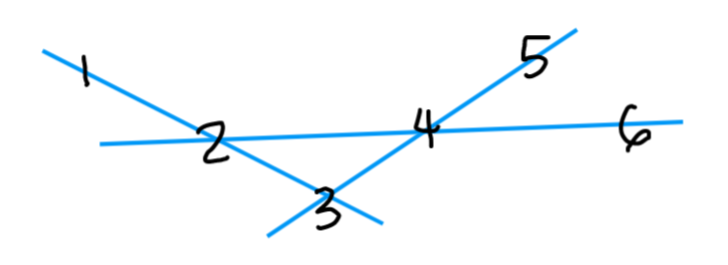
\includegraphics[height=1in]{1.png}
\end{center}

Incidence structures can also be interpreted as edges in a bipartite graph. On one side, your vertices are the elements. On the other side, your vertices are the subsets. An edge joins an element to each subset it belongs to.

The incidence matrix is not a method, just a tool. The method we'll explore is double counting: first {\bfseries \color{RowBlue} counting by rows}, then {\bfseries \color{ColOrange} counting by columns}.

\subsubsection*{Examples}

\begin{enumerate}

\item (Baltic Way 2001) A set of $8$ problems was prepared for an exam. Each student was given $3$ of them. No two students received more than one common problem. What is the maximum number of students?

\textbf{Sketch:} Construct an incidence matrix where columns are problems and rows are students. We want to count the total number of ones.

\cbyrows If there are $s$ students, there are $s$ rows with $3$ each, giving $3s$ in total.

\cbycols We want the number of ones in each column, but we don't know that, so instead we bound. Suppose a column had $4$ ones. Then the rows that had those ones must have $2$ other ones, so there are $8$ more ones among those rows. But no two of these ones can be in the same column, otherwise there would be two students who got two or more common problems. There are only $7$ remaining columns, so this is impossible. Thus, there are at most $3$ ones in each column. There are $8$ columns with at most $3$ each, giving at most $24$ in total.

Thus $3s \le 24$, so $s \le 8$. It remains to find a construction; this isn't too bad.

\textbf{Remark 1:} Please remember how we bounded the number of ones in each column. We won't have another example with this trick, but it will appear several times in the problems.

\textbf{Remark 2:} Here's a cool idea that \textit{almost} works. Construct an incidence matrix where columns are \textit{pairs of problems} and rows are students. An entry would be $1$ if the student was given that pair of problems, and $0$ otherwise. Then each pair of problems could've been given to at most one student, as otherwise two students would've had two common problems. This gives us $3s \le \binom 82$, or $s \le 9$, which isn't a strong enough bound.




\item (China 1996) Eight singers participate in an art festival where several songs are performed. Each song is performed by $4$ singers, and each pair of singers performs together in $\lambda$ songs. Determine the minimum value of $\lambda$.

\textbf{Sketch 1:} Construct an incidence matrix where columns are singers and rows are songs. The trick is to count the number of ``row pairs'' of ones: that is, the number of pairs of ones that lie in the same row. In this case, rows represent songs, so pairs of ones in the same row are pairs of singers performing a song.

\cbyrows Suppose there are $b$ rows. Each row has $4$ ones, giving $6$ row pairs, and $6b$ pairs in total.

\cbycols Pick a pair of columns; there are $28$ of them. Each pair of columns gives $\lambda$ row pairs. This gives $28\lambda$ pairs in total.

Thus $6b = 28\lambda$, so $\lambda \ge 3$. It remains to find a construction; this is actually the painful part.

\textbf{Sketch 2:} We still count row pairs of ones, but this time, we fix a column and count only the pairs that have a one in this column. In other words, we're counting the pairs of singers who sing in the same song, with one of the singers fixed. Suppose this given singer sang $r$ songs.

\cbyrows Suppose the given singer sang $r$ songs. Each of the $r$ songs gives $3$ row pairs, and $3r$ pairs in total.

\cbycols Each of the other $7$ singers sang $\lambda$ songs with this singer, giving $7\lambda$ pairs in total.

Thus $3r = 7\lambda$ and $\lambda \ge 3$; it remains to find a construction.

\textbf{Remark:} For these problems, the write-ups are easier to understand if we don't mention incidence matrices (or rows, or columns) at all. They're just a tool to help us find what to double count.



\item (IMC 2002) Two hundred students participated in a mathematical contest. They had six problems to solve. It is known that each problem was correctly solved by at least $120$ participants. Prove that there must be two participants such that every problem was solved by at least one of these two students.

\textbf{Sketch:} Construct an incidence matrix where columns are problems and rows are students. Assume the opposite. That means each pair of students didn't solve at least one problem. In other words, each pair of rows has at least one column where they're both zero! That means we want to count column pairs of zeroes.

\cbyrows Pick a pair of rows; there are $\binom{200}{2} = 19\,900$ of them. Each pair of rows gives at least one column pair, so at least $19\,900$ in total.

\cbycols Each column has at least $120$ ones, so there are at most $80$ zeroes in each column. There are six columns, so at most $6\binom{80}{2} = 18\,960$ in total.

Combining the two counts gives a contradiction.

\textbf{Remark:} The way I'd write this solution would be as follows. Suppose the contrary. Let $T$ be the number of tuples (student, student, problem), such that there are two distinct students and a problem that neither one solved. Then [\dots\!] so $T \ge 19\,900$. Also [\dots\!] so $T \le 18\,960$. Thus $19\,900 \le T \le 18\,960$, contradiction.



\item In a chess club, $n$ people gathered to play chess against each other, as they pleased. No two people played against each other more than once. At the end of the day, it was observed that a total of $3n$ games had been played. Moreover, if we choose any two players, say $A$ and $B$, there would be at most one other player who had played with both $A$ and $B$. Prove that $n > 30$.

\textbf{Sketch:} Construct an incidence matrix where columns and rows are people. We count the column pairs of ones.

\cbyrows Pick a pair of rows; there are $\binom n2$ of them. Each pair of rows gives at most one column pair, as at most one person played with the people represented by these two rows. There are at most $\binom n2$ column pairs in total.

\cbycols Suppose the $i$th column had $c_i$ ones. Because there are a total of $3n$ games, $\sum c_i = 6n$. Applying Jensen's, we get \[
  \sum_{i = 1}^{n} \binom{c_i}{2} \ge n \binom{ \left( \sum c_i \right)/n }{2} = n \binom{6}{2} = 15n.
\]

Combining the two counts, $15n \le \binom n2$, thus $n \ge 31$ as desired.

\textbf{Remark:} When we can't get good column bounds, we can sometimes assign variables and use Jensen's. Using Jensen's like this is too weak, however, because equality isn't always possible. For example, it's true that $\binom a2 + \binom b2 \ge 2\binom{ \frac{a+ b}{2} }2$. But if $a + b$ is odd, you can get a better lower bound of $\binom{ \frac{a + b - 1}{2} }2 + \binom{ \frac{a + b + 1}{2} }2$.

\end{enumerate}

\subsubsection*{Problems}

\begin{enumerate}

\item (Balanced block designs) Let $A_1, A_2, \ldots, A_b$ be $k$-element subsets of $ S = \left\{ 1, 2, \ldots, v \right\} $. Suppose each pair of elements in $S$ is in exactly $\lambda$ of the $A_i$s. Prove that each element in $S$ is contained in exactly $r$ of the $A_i$s, for $r = \lambda(v-1)/(k-1) = bk/v$. \hint{\ref{h:1}}

\item (Projective planes) Let $n$ and $k$ be integers greater than $1$. Suppose that $A_1, \ldots, A_k$ are $3$-element subsets of $S = \{1, 2, \ldots, n\}$ such that:
\begin{itemize}
  \item for $1 \le i < j \le k$, $|A_i \cap A_j| = 1$, and
  \item for $1 \le \ell < m \le n$, there is exactly one $A_i$ such that $\{\ell, m\} \subseteq A_i$.
\end{itemize}
What are all possible values of $n$?

\item (USA TST 2005) Let $n$ be an integer greater than $1$. For a positive integer $m$, let $S_m = \{1, 2, \ldots, mn\}$. Suppose there exists a $2n$-element set $T$ such that
\begin{enumerate}
  \item each element of $T$ is an $m$-element subset of $S_m$,
  \item each pair of elements of $T$ shares at most one common element, and
  \item each element of $S_m$ is contained in exactly two elements of $T$.
\end{enumerate}
Determine the maximum possible value of $m$ in terms of $n$. \hint{\ref{h:2}}

\item Let $S_1, S_2, \ldots, S_{5n}$ be subsets of $A = \left\{ 1, 2, \ldots, 100 \right\} $ such that every element of $A$ appears in exactly $4n$ of the $S_i$s. Prove there exists $i, j, k$ such that $S_i \cup S_j \cup S_k = A$.

\item (China 1994?) Let $A_1, A_2, \ldots, A_k$ be $5$-element subsets of $S = \left\{ 1, 2, \ldots, 10 \right\} $ such that $|A_i \cap A_j| \le 2$ for $1 \le i < j \le k$. Find the maximum value of $k$. \hint{\ref{h:3}}

\item (China TST 1992) Sixteen students took part in a math competition where every problem was a multiple choice question with four choices. After the contest, it is found that any two students had at most one answer in common. Determine the maximum number of questions. \hint{\ref{h:3}}

\item (IMO 1998) In a competition, there are $a$ contestants and $b$ judges, where $b \ge 3$ is an odd integer. Each judge rates each contestant as either ``pass'' or ``fail''. Suppose $k$ is a number such that for any two judges, their ratings coincide for at most $k$ contestants. Prove that \[
  \frac{k}{a} \ge \frac{b-1}{2b}.
\]

\item (USA 2011) Let $X$ be a set with $|X| = 225$. Suppose further there are eleven subsets $A_1, \ldots, A_{11}$ of $X$ such that $|A_i| = 45$ for $1 \le i \le 11$ and $|A_i \cap A_j| = 9$ for $1 \le i < j \le 11$. Prove that $|A_1 \cup \dots \cup A_{11}| \ge 165$, and give an example for which equality holds. \hint{\ref{h:2}}

\end{enumerate}

\subsubsection*{Harder problems}

\begin{enumerate}[resume]

\item (Singapore 2010) Let $n$ be a positive integer. Find the smallest positive integer $k$ with the property that for any coloring of the squares of a $2n \times k$ chessboard with $n$ colors, there are $2$ columns and $2$ rows such that the $4$ squares in their intersections have the same color. \hint{\ref{h:4}}

\item (USA 1979) An organization has $n$ members, and it has $n + 1$ distinct three-member committees. Prove that there are two committees that share exactly one member. \hint{\ref{h:5}}

\item (Singapore 2006) Let $n$ be a positive integer. Let $S_1, S_2, \ldots, S_k$ be a collection of $2n$-element subsets of $ \left\{ 1, 2, \ldots, 4n -1, 4n \right\} $ so that $S_i \cap S_j$ contains at most $n$ elements for all $1 \le i < j \le k$. Show that $k \le 6^{(n+1)/2} $. \hint{\ref{h:6}}

\item (USA 1984) A math exam has two papers, where each paper consists of at least one question and both papers have $28$ questions altogether. Each pupil attempted $7$ questions. Each pair of questions was attempted by exactly two pupils. Show that one pupil attempted either zero or at least four questions in the first paper. \hint{\ref{h:7}}

\item (China 1993) A group of $10$ people went to a bookstore. It is known that everyone bought exactly $3$ books, and for every two people, there is at least one book that both of them bought. What is the least number of people that could have bought the book purchased by the greatest number of people? \hint{\ref{h:8}}

% \item (China TST 1995) Twenty-one people took a test with $15$ true-or-false questions. It is known that for every two people, there is at least one question they both have answered correctly. Determine the minimum possible number of people that could have correctly answered the question that most number of people are correct on.

\item (IMO 2001) Twenty-one girls and twenty-one boys took part in a mathematical competition. It turned out that each contestant solved at most six problems, and for each pair of a girl and a boy, there was at least one problem that was solved by both the girl and the boy. Show that there is a problem that was solved by at least three girls and at least three boys. \hint{\ref{h:9}}

\item (IMO 2005) In a mathematical competition $6$ problems were posed to the contestants. Each pair of problems was solved by more than $\frac25$ of the contestants. Nobody solved all $6$ problems. Show that there were at least $2$ contestants who solved exactly $5$ problems.

\end{enumerate}

\subsubsection*{Hints}

\begin{enumerate}
\item \label{h:6} Use Remark 2 from the first example.
\item \label{h:7} How many students are there? How many problems did each solve?
\item \label{h:4} The case $n = 4$ is similar to the China TST 1992 problem.
\item \label{h:1} This generalizes the second example.
\item \label{h:3} For the construction, try to put things into sets greedily, and that'll probably work.
\item \label{h:5} Induct on $n$.
\item \label{h:8} First show the answer is at least $4$. Then show it can't be $4$.
\item \label{h:9} Bound triplets of matching problems in rows and columns.
\item \label{h:2} For the construction, represent something geometrically, like the figure on page $1$.
\end{enumerate}

\subsubsection*{Sketches}

\begin{enumerate}

\item We count row pairs of ones, where one of the ones is in a given column. \cbyrows If the given column has $r$ ones, each gives $k-1$ pairs along its row. \cbycols If we pick one of the other $v-1$ columns, there are $\lambda$ rows that contain a pair. Thus $r(k-1) = \lambda(v-1)$. The $bk = vr$ follows from counting all the ones.

\textbf{Remark:} Note that $v$, $k$, and $\lambda$ determine $b$ and $r$. We call the family of subsets a $2$-balanced design, because the subsets are balanced with respect to the $2$-element subsets of $S$. We want to prove that every $2$-balanced design is also $1$-balanced. In fact, for every $s < t$, every $t$-balanced design is also $s$-balanced; the proof is similar.

\item This is a special case of the previous problem. We see that $r = \frac{n-1}2 = \frac{3k}{n}$. We then count column pairs of ones. \cbyrows Each pair of rows gives one, so $\binom k2$. \cbycols Each column has $\binom r2$ pairs, giving $n\binom r2$. All the info gives $n = 7$. The construction is given by the \href{https://en.wikipedia.org/wiki/Fano_plane}{Fano plane}.

\textbf{Remark:} Note that each set contains $3$ points and each point is in $3$ sets. For every prime power $p^n$, there's a similar construction with the $3$ in the problem replaced with $p^n + 1$; these are known as the finite projective planes. It's unknown whether there's a finite projective plane not of this form.

\item We count column pairs of ones. \cbyrows There are $ \binom{2n}{2} $ pairs of rows, and each pair of row has at most one pair. \cbycols Each of the $mn$ columns has exactly two ones. Thus $mn \le \binom{2n}{2}$, so $m \le 2n - 1$. It remains to find a construction; consider $2n$ lines in general position.

\item Assume otherwise; we count column triplets of zeroes. \cbyrows There are $\binom{5n}{3}$ triplets of rows, each giving at least one column pair. \cbycols Each column has $n$ zeroes, giving $100 \binom{n}{3}$ triplets. Thus $\binom{5n}{3} \le 100 \binom{n}{3}$, contradiction after some algebra.

\item We count column pairs of ones. \cbyrows There are $\binom{k}{2}$ pairs of rows, each giving at most two column pairs. \cbycols The total number of ones is $5k$, so by Jensen, there are $\sum \binom{c_i}{2} \ge 10 \binom{k/2}{2}$ column pairs. Thus $10\binom{k/2}{2} \le 2\binom{k}{2}$, so $k \le 6$. It remains to find a construction, e.g. 01234, 01567, 02589, 13689, 24679, 34578.

\item Construct the incidence matrix where columns are problems, rows are students, and entries are the students' answers. We count column pairs of matching answers. \cbyrows There are $\binom{16}{2}$ pairs of rows, each giving at most one pair. \cbycols Suppose there are $p$ columns. By Jensen, each column gives at least $4\binom42$ pairs. Thus $4p\binom42 \le \binom{16}{2}$, so $p \le 5$. It remains to find a construction; consider families of parallel lines in $\mathbb{F}_4 \times \mathbb{F}_4$.

\item Construct the incidence matrix where columns are contestants and rows are judges. We count column pairs of matching ratings. \cbyrows There are $\binom b2$ pairs of rows, each giving at most $k$ pairs. \cbycols By Jensen, each of the $a$ columns gives at least $\binom{(b-1)/2}{2} + \binom{(b+1)/2}{2} = (b-1)^2/4$ pairs. Combining, we get $a(b-1)^2/4 \le k\binom b2$, as desired.

\item We count column pairs of ones. \cbyrows There are $\binom{11}{2}$ pairs of rows, each giving $9$ column pairs. \cbycols Suppose there are $n$ columns, and that the $i$th column had $c_i$ ones. There are a total of $45 \times 11$ ones. By Jensen, we get $\sum \binom{c_i}{2} \ge n\binom{495/n}{2}$. Combining, we get $9\binom{11}{2} \ge n\binom{495/n}{2}$, or $n \ge 165$. It remains to find a construction; consider $11$ planes in general position.

\end{enumerate}

\subsubsection*{References}

Problems were mostly lifted from Loh's \href{https://www.math.cmu.edu/~lohp/docs/math/mop2011/combin-sets.pdf}{Combinatorics of Sets} handout, Shi-Jie's \href{https://www.scribd.com/document/87289070/HCMOP-Open-Incidence-Matrix-Solutions}{Incidence Matrix} handout, and Zhao's \href{https://yufeizhao.com/olympiad/doublecounting_mop.pdf}{Double Counting} handout.

\end{document}


(Iran 2010) A school has $n$ students and some classes. Each student can participate in any number of classes. Every class has at least two students participating. If two different classes have at least two common students, then the number of the students are distinct. Prove that the number of classes is at most $\left(n-1\right)^2$.

(Hong Kong 2007) In a school there are $2007$ girls and $2007$ boys. Each student joins no more than $100$ clubs in the school. It is known that any two students of opposite genders have joined at least one common club. Show that there is a club with at least $11$ boys and $11$ girls.

---

Let $k > 1$ be an integer, and suppose that $A_1, \ldots, A_k$ are $3$-element subsets of $S = \{1, 2, \ldots, n\}$ such that:
\begin{itemize}
  \item for $1 \le i < j \le k$, $|A_i \cap A_j| = 1$, and
  \item for $1 \le \ell < m \le n$, there is exactly one $A_i$ such that $\{\ell, m\} \subseteq A_i$.
\end{itemize}
What are all possible values of $n$?
